\documentclass[tikz]{standalone}

\usepackage{amsmath}
\usetikzlibrary{calc,angles,quotes}

\renewcommand{\vec}[1]{\boldsymbol{#1}}

\tikzset{>=latex}
\begin{document}
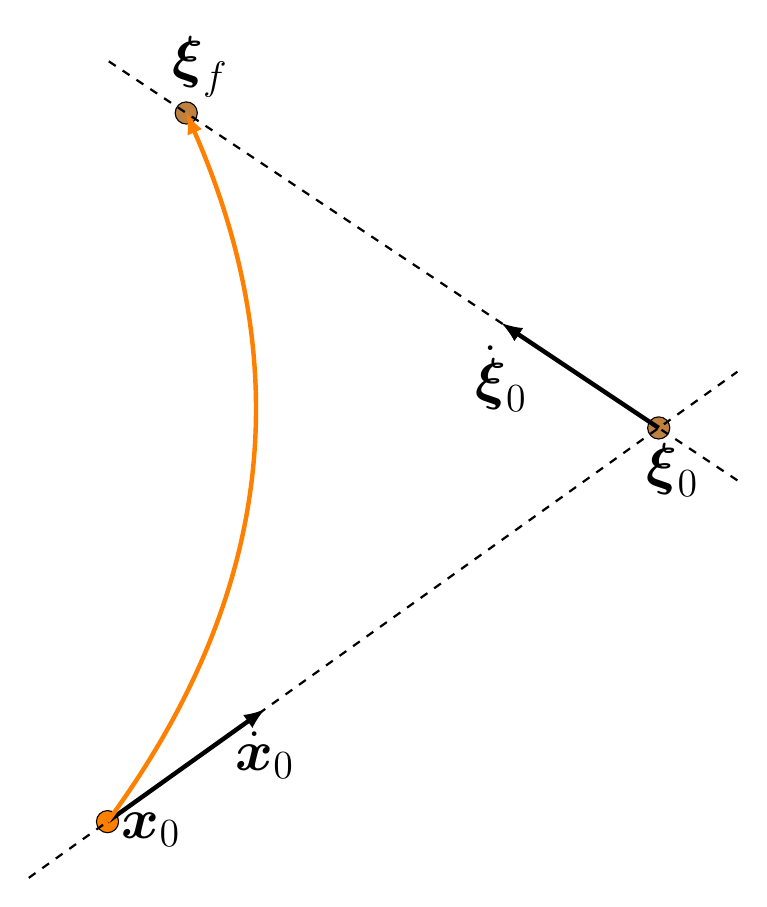
\begin{tikzpicture}

  \node[coordinate] (x_init) at (-1,-0.714) {};
  \node[coordinate] (x0) at (0,0) {};
  \node[coordinate] (cp_0) at (7,5) {};
  \node[coordinate] (cp_0_final) at (8,5.7142) {};
  \node[coordinate] (cp_0_init) at (8,4.3333) {};
  \node[coordinate] (cp_f) at (1,9) {};
  \node[coordinate] (cp_f_final) at (0,9.6667) {};

  
  \draw[black, fill=brown] (cp_0) circle (4pt);
  \draw[black, fill=brown] (cp_f) circle (4pt);
  \draw[black, fill=orange] (x0) circle (4pt);

  \node[right=5, below = 2] at (cp_0) {\huge $\vec{\xi}_{0}$};
  \node[right=5, above = 2] at (cp_f) {\huge $\vec{\xi}_{f}$};
  
  
  \draw[-,thick, dashed] (x_init)  --(cp_0_final);
  \draw[-,thick, dashed] (cp_0_init)  -- (cp_f_final);

  \draw[->,ultra thick] (x0) node[below = 3, right = 1]{\huge $\vec{x}_{0}$}  -- (2, 1.428) node[right, below = 4]{\huge $\dot{\vec{x}}_{0}$};


    \draw[->,ultra thick] (cp_0)  -- (5, 6.3333) node[right, below = 4]{\huge $\dot{\vec{\xi}}_{0}$};

  \draw[->, ultra thick, orange](x0) to [bend right,looseness=1]  (cp_f);
  
  
\end{tikzpicture}
\end{document}
